\section{Evaluation}
We first applied our approaches to several real-world dataset and compare our method with the uniform random sampling. Then we conduct several user studies on specific analysis tasks. 
\subsection{Experimental results}
In this section, we evaluate our method by presenting the applications on three taxi trajectory datasets: Porto, Shenzhen and Chengdu. We compare the visualization among the full dataset, random sampling and the proposed method from different levels of details. 
\subsubsection{Case of Porto Distinct}
Our first example uses taxi trajectories collected from 442 active taxis in the city of Porto distinct, Portugal~\footnote{\url{http://www.geolink.pt/ecmlpkdd2015-challenge/dataset.html}}. The trajectories cover several cities in and around the Porto distinct.

\textbf{Spatial coverage of overview.}
Figure~\ref{fig:teaser} A - F show the top level trajectory visualization of different approaches and the parameter settings. Figure~\ref{fig:teaser} C present the visualization generated by the whole dataset, from which we can get an overview of the movement patterns in Porto district. For example, many trajectories are concentrated in the center of the figure(shown around point Figure\ref{fig:teaser}C$_1$) indicating that the most taxi activities are around the \UC{Porto City}. In addition, the many other regions with dense trajectory cluster also indicate the location of the cities in the Porto district(shown as the dash circle in Figure~\ref{fig:teaser} C). Figure~\ref{fig:teaser} B and E depict the visualization generated by uniform random sampling and $\avats$ respectively. Both of these two sampling methods take 0.01 as the sampling rate. The uniform random sampling almost only preserves the visual elements around the Porto City. Figure~\ref{fig:teaser} depicts visualization generated by $\avats$, which looks the same as the whole dataset. Not only the Porto City but also the margin city patterns are preserved, which are shown as the dash circles in ~\ref{fig:teaser} E. Another important factor affecting the visual fidelity of sampling results is the sampling rate. Figure\ref{fig:teaser} B and C show the sampling results of random method with sampling rate set as 0.01 and 0.001. With the decreasing of the sampling rate, the shape of the trajectory visualizations clearly shrink to the Porto City. Figure\ref{fig:teaser} E and D demonstrate the visualization of $\avats$ with the sampling rate of 0.01 and 0.001, from which we observe that when the sampling rate is decreased, the framework of the trajectories is preserved while the trajectories around Porto City are significantly removed since more \QM{blank space/gap} can be found in the center of figure as shown in Figure~\ref{fig:teaser} D$_1$. Figure~\ref{fig:teaser} F shows the visualization generated by $\avats$ with color encoding where the \QM{representativeness} of a trajectory is encoded by color. As shown by Figure~\ref{fig:teaser} E$_1$, no clear pattern can be found due to the dense concentration of massive trajectories. While in Figure~\ref{fig:teaser} F$_1$, some trajectories with high representative score are highlighted by dark orange color such as F$_2$ in Figure~\ref{fig:teaser} F, which indicates \QM{road name}, a main street in Porto City. From the overview, $\avats$ can preserve the general structure very well in the comparison with uniform random sampling, and more information of the movement can be visualized with color encoding.

$\avats$ outperforms the uniform random sampling in the visualization of overview. Then we evaluate the performance of $\avats$ at different level of details. We first select several regions of interest as shown in the Figure\ref{fig:porto} A. 
Region R3 is far away from Porto City and contains two other cities: Paredes and Penafiel. Region R3 has very few trajectories as shown in Figure~\ref{fig:porto} D$_1$. Figure~\ref{fig:porto} D$_1$ to D$_4$ show the visualization in region 3 at level 11.  Compare with the visualization of full dataset, the random sampling almost misses all trajectories in this region(as shown in Figure~\ref{fig:porto} D$_2$). While $\vats$ samples much more trajectories than random sampling as shown in Figure~\ref{fig:porto} D$_3$. However, some meaningful trajectories are still missing such as the trajectory bundle shown in Figure~\ref{fig:porto} h, which is laid in on the road \QM{road name} connecting the two cities of Paredes and Penafiel. Further more, the trajectory structure of city Penafiel is not precisely preserved(shown as region g in Figure~\ref{fig:porto} D$_3$ i) because some  trajectory branches are missed.  
By setting the representative parameter as 64, $\avats$ generate a more confidential visualization than $\vats$. 

There are three cities located in the region R2 including Ermesinde, Rio Tinto and Valongo. Region 2 is near to the center of Porto and there are more taxi trajectories. 
Figure~\ref{fig:porto} C$_2$ and C$_3$ present the visualization generated by $\avats$ with the representative parameters are set as 4 and 64. We observe that the visualization shown in Figure~\ref{fig:porto} C$_3$ have more details trajectory branches than Figure~\ref{fig:porto} C$_3$(as shown in region d of Figure~\ref{fig:porto} C$_2$ and C$_3$). In this case, a larger representative parameter is more beneficial in preserving the details at this level. Furthermore, Figure~\ref{fig:porto} C$_4$ shows the visualization of $\avats$($delta = 64$) with color encoding. In the comparison with Figure~\ref{fig:porto} C$_3$, the visualization in Figure~\ref{fig:porto} further highlights the movement distribution, for instance, city Rio Tinto has more taxi activities than other two cities because region f in Figure~\ref{fig:porto} has more dark colored trajectories than region e and g.

The region R1 is the center of Porto city, which has the highest concentration of the trajectories and cause serious visual clutter if all trajectories are visualized(as shown in Figure\ref{fig:porto} B$_1$). $\avats$($delta = 4$) greatly alleviates the visual clutter and preserves the framework which basically follows the road network as shown in Figure~\ref{fig:porto} B$_2$. Furthermore, when setting the representative parameter $delta$ as 64, the structure is further \QM{clarified} as shown in region b of Figure~\ref{fig:porto} B$_3$ and B$_4$, and have more trajectory details than $\avats$($delta = 4$) as shown in region a of Figure~\ref{fig:porto} B$_2$ and B$_3$.
 
\begin{figure*}[t]
	\centering
	\vspace{2mm}
	\includegraphics[width=0.98\textwidth]{pictures/experiment_study/case_porto.pdf}
	\caption{Visualization at dense and sparse region respectively.}
	\vspace{0mm}
	\label{fig:porto}
\end{figure*}

\begin{figure}[t]
	\centering
	\vspace{2mm}
	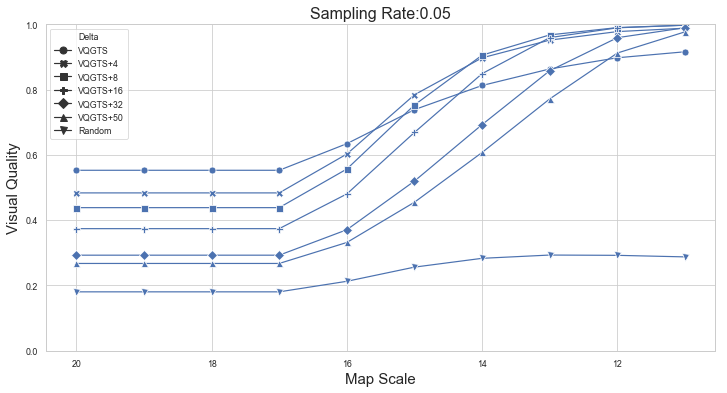
\includegraphics[width=0.45\textwidth]{pictures/experiment_study/quanlity.png}
	\caption{Visual quality chart. X axis indicates map scale from detail view to overview; y axis indicate the visual quality. }
	\vspace{0mm}
	\label{fig:quality_chart}
\end{figure}


\subsubsection{Shenzhen Trajectories}
We further evaluate the proposed approach using the taxi trajectories of Shenzhen, which includes 428K trajectories collected from \QM{**} taxis in one day. All the cases generated by sampling methods set the sampling rates as 0.01. Figure~\ref{fig:shenzhen} A-D present the overview generated by whole dateset, random sampling, $\avats$ and $\avats$ with color encoding. At the top level, the visualization of raw dataset(Figure~\ref{fig:shenzhen} A) shows the most taxi trajectories are recorded in source districts of Shenzhen, including Baoan, Nanshan, Futian and Luohu districts, which are commercial zones of Shenzhen. Figure ~\ref{fig:shenzhen} B demonstrates the trajectories generated by random sampling, we observe that the most of the trajectories sampled by random methods are located at these regions where most the taxi activities concentrate. On the other hand, the trajectories at the north Shenzhen are missing, thus making the visualization visually different from the whole dataset.
$\avats$ outperforms random method by guaranteeing the spatial coverage of the whole trajectories thus making the visualization visually close to the whole dataset. Further more, some isolate trajectories are still preserved shown in Figure~\ref{fig:shenzhen} C. $\avats$ with color is further improved to reveal spatial distribution of the trajectories. For example, for the regions a, b of Figure~\ref{fig:shenzhen} A and C, the visualization is unable to explain which region has more taxi activities because both of these two regions are fully covered by trajectories. In Figure~\ref{fig:shenzhen} D, we find the overall color of region a is darker than region b, which indicates more trajectories can be found in region a than region b. 

Then we narrow down to the region of airport shown as Figure~\ref{fig:shenzhen} E,F,G and H. Clearly the random sampling totally misses the overview of the trajectories.  Both $\avats$ and $\avats$ with color encoding can present the trajectory framework intuitively. The $\avats$ with color encoding further enriches the information by encoding the trajectory with color. For example, more trajectories pass through G4 and G104 thab Baoan Avenue, which is hard to discovered from the Figure~\ref{fig:shenzhen} E, F and G.  

Similarly, in the region near to the Shenzhen North Railway Station, the visualization generated by $\avats$ can reveals some road structure such as the \QM{round entrance to the motorway} shown as region c in Figure~\ref{fig:shenzhen} K. With the color encoding, we can also easily discover that the road G94 have a higher road traffic flow than the Minzhi avenue and Mellon avenue, which is hard to discovered from Figure~\ref{fig:shenzhen} I, G and K.

\begin{figure*}[t]
	\centering
	\vspace{2mm}
	\includegraphics[width=0.98\textwidth]{pictures/experiment_study/case_shenzhen.pdf}
	\caption{Case study of Shenzhen.}
	\vspace{0mm}
	\label{fig:shenzhen}
\end{figure*}



\subsection{Expert overview}

